
\subsection{Answers}
\begin{table}[htb]%
\begin{center}%
\caption{Q14: How do you check MPI specifications when you are writing MPI programs?}%
\label{tab:Q14-ans}%
\begin{tabular}{l|l|r}%
\hline%
Choice & Abbrv. & \# Answers \\%
\hline%
{\small I read online documents (such as man pages).} & Online docs & 579 (68.8\%) \\%
{\small I search the Internet (Google / Stack Ov$\cdots$} & Internet & 566 (67.2\%) \\%
{\small I read the MPI Standard document (web/book).} & MPI standard & 430 (51.1\%) \\%
I ask colleagues. & Colleagues & 188 (22.3\%) \\%
{\small I read book(s) (except the MPI standard).} & Books & 108 (12.8\%) \\%
I know almost all MPI routines. & I know all & 46 (5.5\%) \\%
other & - & 11 (1.3\%) \\%
\hline%
\multicolumn{2}{c}{total} & 1928 (842)\\%
\hline%
\end{tabular}%
\end{center}%
\end{table}%

\clearpage%
{\footnotesize\begin{landscape}%
\begin{longtable}[htb]{r|c|c|c|c|c|c|c|c|c|c}%
\caption{Q14: How do you check MPI specifications when you are writing MPI programs?}%
\label{tab:Q14-mans} \\%
\hline%
Multi-Answer & overall & FR & GR & IT & UK & eu & JP & RU & US & others \\
 \hline%
\endfirsthead%
\multicolumn{11}{r}{(continued from the previous page)}\\%
\hline%
Multi-Answer & overall & FR & GR & IT & UK & eu & JP & RU & US & others \\
 \hline%
\endhead%
\hline%
(total) & 842 & 124 & 157 & 57 & 66 & 141 & 64 & 93 & 58 & 82 \\%
\hline%
\multicolumn{11}{r}{(continue to the next page)}\\%
\endfoot%
\hline%
(total) & 842 & 124 & 157 & 57 & 66 & 141 & 64 & 93 & 58 & 82 \\%
\hline%
\endlastfoot%
\hline%
{Online docs, Internet} & 144 & 26 & 18 & 12 & 15 & 27 & 9 & 15 & 9 & 13 \\%
{MPI standard, Online docs, Internet} & 110 & 11 & 30 & 8 & 6 & 20 & 7 & 14 & 5 & 9 \\%
{Online docs} & 75 & 14 & 3 & 7 & 8 & 13 & 8 & 4 & 8 & 10 \\%
{MPI standard} & 73 & 7 & 23 & 5 & 1 & 7 & 6 & 11 & 7 & 6 \\%
{Internet} & 61 & 9 & 4 & 4 & 6 & 12 & 8 & 6 & 2 & 10 \\%
{Online docs, Colleagues, Internet} & 53 & 7 & 14 & 4 & 2 & 15 & 1 & 4 & 2 & 4 \\%
{MPI standard, Online docs} & 47 & 8 & 12 & 3 & 2 & 7 & 4 & 3 & 4 & 4 \\%
{MPI standard, Internet} & 37 & 3 & 10 & 3 & 2 & 8 & 5 & 2 & 3 & 1 \\%
{MPI standard, Online docs, Colleagues, Internet} & 36 & 8 & 8 & 1 & 2 & 7 & 2 & 6 & 2 & 0 \\%
{MPI standard, Colleagues, Internet} & 18 & 3 & 8 & 1 & 1 & 0 & 1 & 2 & 0 & 2 \\%
{MPI standard, Books, Online docs, Colleagues, Internet} & 17 & 1 & 1 & 3 & 4 & 2 & 1 & 1 & 3 & 1 \\%
{MPI standard, Books, Online docs, Internet} & 15 & 1 & 3 & 0 & 2 & 1 & 2 & 1 & 2 & 3 \\%
{Colleagues, Internet} & 13 & 3 & 5 & 2 & 0 & 2 & 0 & 1 & 0 & 0 \\%
{Books, Online docs, Internet} & 11 & 4 & 1 & 1 & 0 & 0 & 2 & 3 & 0 & 0 \\%
{MPI standard, Online docs, Internet, I know all} & 10 & 2 & 0 & 0 & 0 & 1 & 0 & 3 & 4 & 0 \\%
{Colleagues} & 9 & 0 & 0 & 0 & 0 & 2 & 1 & 3 & 0 & 3 \\%
{MPI standard, Books, Online docs} & 9 & 0 & 3 & 0 & 1 & 0 & 1 & 2 & 0 & 2 \\%
{MPI standard, Books, Internet} & 8 & 1 & 0 & 0 & 0 & 1 & 1 & 2 & 1 & 2 \\%
{Books, Online docs, Colleagues, Internet} & 8 & 1 & 0 & 0 & 1 & 2 & 0 & 2 & 1 & 1 \\%
{Books} & 8 & 0 & 0 & 0 & 0 & 0 & 0 & 2 & 0 & 6 \\%
{MPI standard, Books} & 8 & 0 & 1 & 0 & 0 & 2 & 3 & 0 & 1 & 1 \\%
{MPI standard, Books, Online docs, Colleagues, Internet, I know all} & 7 & 0 & 0 & 0 & 7 & 0 & 0 & 0 & 0 & 0 \\%
{MPI standard, Online docs, Colleagues} & 6 & 1 & 2 & 0 & 1 & 1 & 0 & 1 & 0 & 0 \\%
{MPI standard, I know all} & 5 & 0 & 0 & 1 & 0 & 2 & 0 & 0 & 1 & 1 \\%
{Online docs, Colleagues} & 5 & 3 & 0 & 1 & 1 & 0 & 0 & 0 & 0 & 0 \\%
{MPI standard, Online docs, I know all} & 5 & 1 & 1 & 0 & 0 & 2 & 0 & 1 & 0 & 0 \\%
{I know all} & 4 & 0 & 2 & 0 & 0 & 0 & 0 & 0 & 1 & 1 \\%
{Books, Internet} & 4 & 1 & 0 & 0 & 1 & 0 & 0 & 2 & 0 & 0 \\%
{MPI standard, Online docs, Colleagues, Internet, I know all} & 3 & 1 & 2 & 0 & 0 & 0 & 0 & 0 & 0 & 0 \\%
{Books, Online docs} & 3 & 0 & 0 & 0 & 0 & 1 & 0 & 0 & 1 & 1 \\%
{MPI standard, Colleagues} & 3 & 2 & 0 & 0 & 1 & 0 & 0 & 0 & 0 & 0 \\%
{Online docs, I know all} & 2 & 0 & 0 & 0 & 0 & 2 & 0 & 0 & 0 & 0 \\%
{MPI standard, Books, Online docs, Colleagues} & 2 & 1 & 0 & 0 & 0 & 0 & 1 & 0 & 0 & 0 \\%
{Books, Online docs, I look at my existing code} & 1 & 0 & 0 & 0 & 0 & 0 & 0 & 0 & 1 & 0 \\%
{I read the school lectures} & 1 & 0 & 0 & 0 & 0 & 1 & 0 & 0 & 0 & 0 \\%
{manpage} & 1 & 0 & 0 & 0 & 0 & 1 & 0 & 0 & 0 & 0 \\%
{I do not write any} & 1 & 0 & 0 & 0 & 0 & 1 & 0 & 0 & 0 & 0 \\%
{Online docs, Internet, I know all} & 1 & 0 & 0 & 0 & 0 & 0 & 0 & 1 & 0 & 0 \\%
{I don't write MPI programs yet} & 1 & 0 & 0 & 0 & 0 & 1 & 0 & 0 & 0 & 0 \\%
{Internet, I know all} & 1 & 1 & 0 & 0 & 0 & 0 & 0 & 0 & 0 & 0 \\%
{MPI standard, Online docs, Internet, mpi must be CUDA-AWARE. We have 1024 GPUs} & 1 & 0 & 0 & 0 & 0 & 0 & 0 & 1 & 0 & 0 \\%
{MPI standard, Books, Internet, I know all} & 1 & 0 & 0 & 1 & 0 & 0 & 0 & 0 & 0 & 0 \\%
{MPI standard, Online docs, compiler warnings} & 1 & 0 & 1 & 0 & 0 & 0 & 0 & 0 & 0 & 0 \\%
{MPI standard, Online docs, Colleagues, I know all} & 1 & 0 & 1 & 0 & 0 & 0 & 0 & 0 & 0 & 0 \\%
{Books, Online docs, Internet, I know all} & 1 & 1 & 0 & 0 & 0 & 0 & 0 & 0 & 0 & 0 \\%
{MPI standard, Books, Online docs, I know all} & 1 & 0 & 1 & 0 & 0 & 0 & 0 & 0 & 0 & 0 \\%
{Online docs, Lecture notes/preexisting source code} & 1 & 1 & 0 & 0 & 0 & 0 & 0 & 0 & 0 & 0 \\%
{MPI standard, Books, Colleagues} & 1 & 0 & 0 & 0 & 0 & 0 & 1 & 0 & 0 & 0 \\%
{MPI standard, Colleagues, Internet, I know all} & 1 & 0 & 1 & 0 & 0 & 0 & 0 & 0 & 0 & 0 \\%
{MPI standard, Online docs, Colleagues, Internet, I am quite familiar with part of the MPI routines} & 1 & 1 & 0 & 0 & 0 & 0 & 0 & 0 & 0 & 0 \\%
{Colleagues, Internet, I know all} & 1 & 1 & 0 & 0 & 0 & 0 & 0 & 0 & 0 & 0 \\%
{MPI standard, Books, Online docs, Internet, MUST} & 1 & 0 & 0 & 0 & 1 & 0 & 0 & 0 & 0 & 0 \\%
{Online docs, Colleagues, I know all} & 1 & 0 & 0 & 0 & 0 & 0 & 0 & 0 & 0 & 1 \\%
{MPI standard, Books, Colleagues, Internet} & 1 & 0 & 0 & 0 & 1 & 0 & 0 & 0 & 0 & 0 \\%
{I don't write MPI programs} & 1 & 0 & 1 & 0 & 0 & 0 & 0 & 0 & 0 & 0 \\%
{MPI standard, Books, Colleagues, Internet, I know all} & 1 & 0 & 1 & 0 & 0 & 0 & 0 & 0 & 0 & 0 \\%
\hline%
\end{longtable}%
\end{landscape}}%
\clearpage%


\subsection{List of other answers}
\begin{itemize}
\item Europe:France: I am quite familiar with part of the MPI routines
\item Europe:France: Lecture notes/preexisting source code
\item Europe:Germany: I don't write MPI programs
\item Europe:Germany: compiler warnings
\item Europe:UK: MUST
\item Europe:others: I do not write any
\item Europe:others: I don't write MPI programs yet
\item Europe:others: I read the school lectures
\item Europe:others: manpage
\item Russia: mpi must be CUDA-AWARE. We have 1024 GPUs
\item USA: I look at my existing code

\end{itemize}

\begin{figure}[htb]
\begin{center}
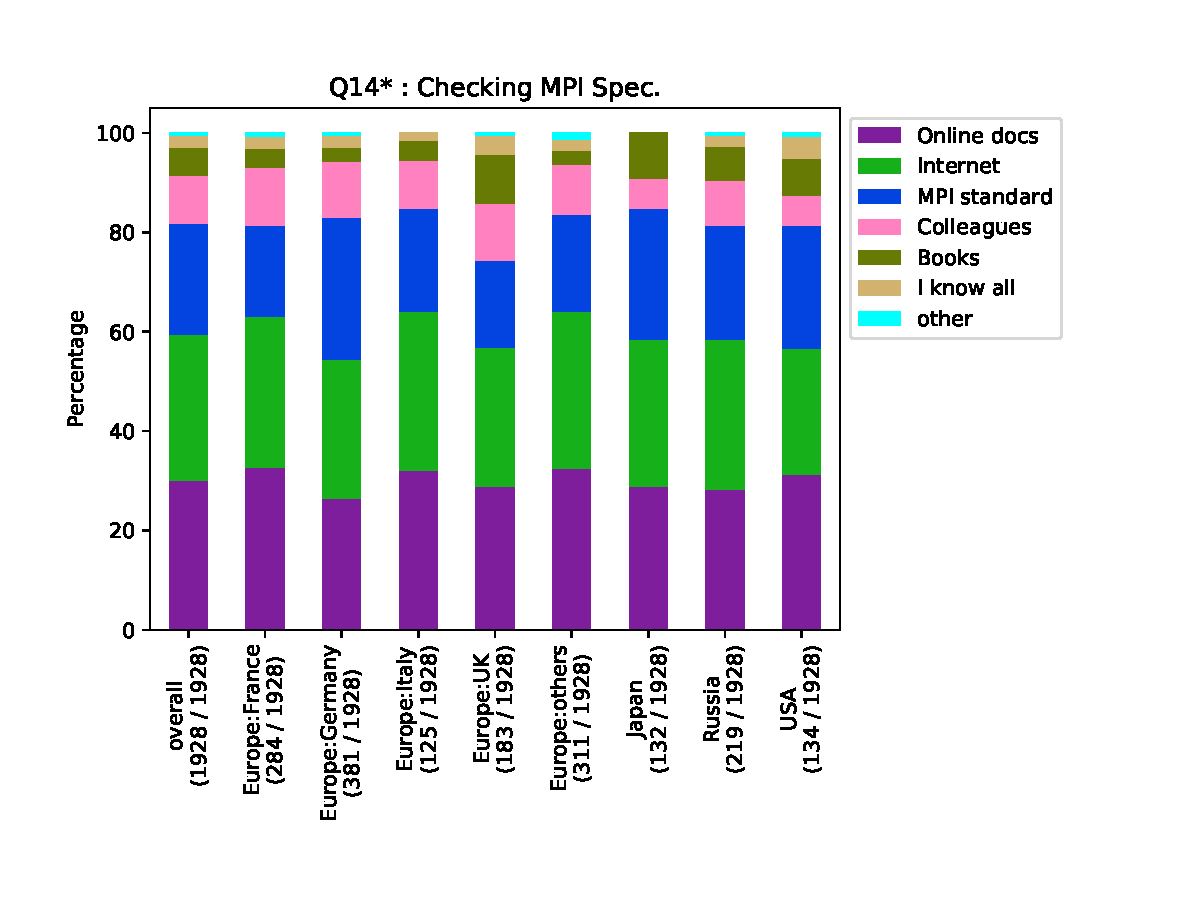
\includegraphics[width=10cm]{../pdfs/Q14.pdf}
\caption{Simple analysis: Q14}
\label{fig:Q14}
\end{center}
\end{figure}

\subsection{Comments}
The most common ways in getting information about MPI specification is to use
either online resources (such as man pages) or to search the Internet. The
common, point with these two sources of information is that they are
dematerialize, which is the common way of working for many developers nowadays.   

Surprisingly, reading the standard (either on the web or with a book) seems to
be quite common as well (20\% of the answers). Last there is no real differences
between regions meaning that the common practice are shared among all the
users. 

% This is the question where the differences among countries/regions are
% hard to see.  I am surprised at that around 20 \% of people are
% reading MPI standard! 
